\chapter{LHC-ATLAS Experiment}
\label{chapter:LHC_ATLAS_experiment}

\section{Large Hadron Collider}
\label{sec:lhc}

The European Organisation for Nuclear Research (CERN) is an international particle-physics laboratory located near Geneva on the border between France and Switzerland.
Since its foundation in 1954, CERN has developed and operated a chain of accelerators and experimental facilities to study the fundamental constituents of matter and their interactions~\cite{CERNAbout}.
The Large Hadron Collider~(LHC) is the largest and highest-energy particle collider in the CERN accelerator complex.
It is installed in the former Large Electron--Positron Collider~(LEP) tunnel, which has a circumference of about $27~\mathrm{km}$ and lies between approximately $45~\mathrm{m}$ and $170~\mathrm{m}$ below the surface~\cite{Evans2008LHC,CERNLHC}.
A schematic overview of the LHC ring and its interaction points is shown in Fig.~\ref{fig:lhc_layout}.

\begin{figure}[htbp]
    \centering
    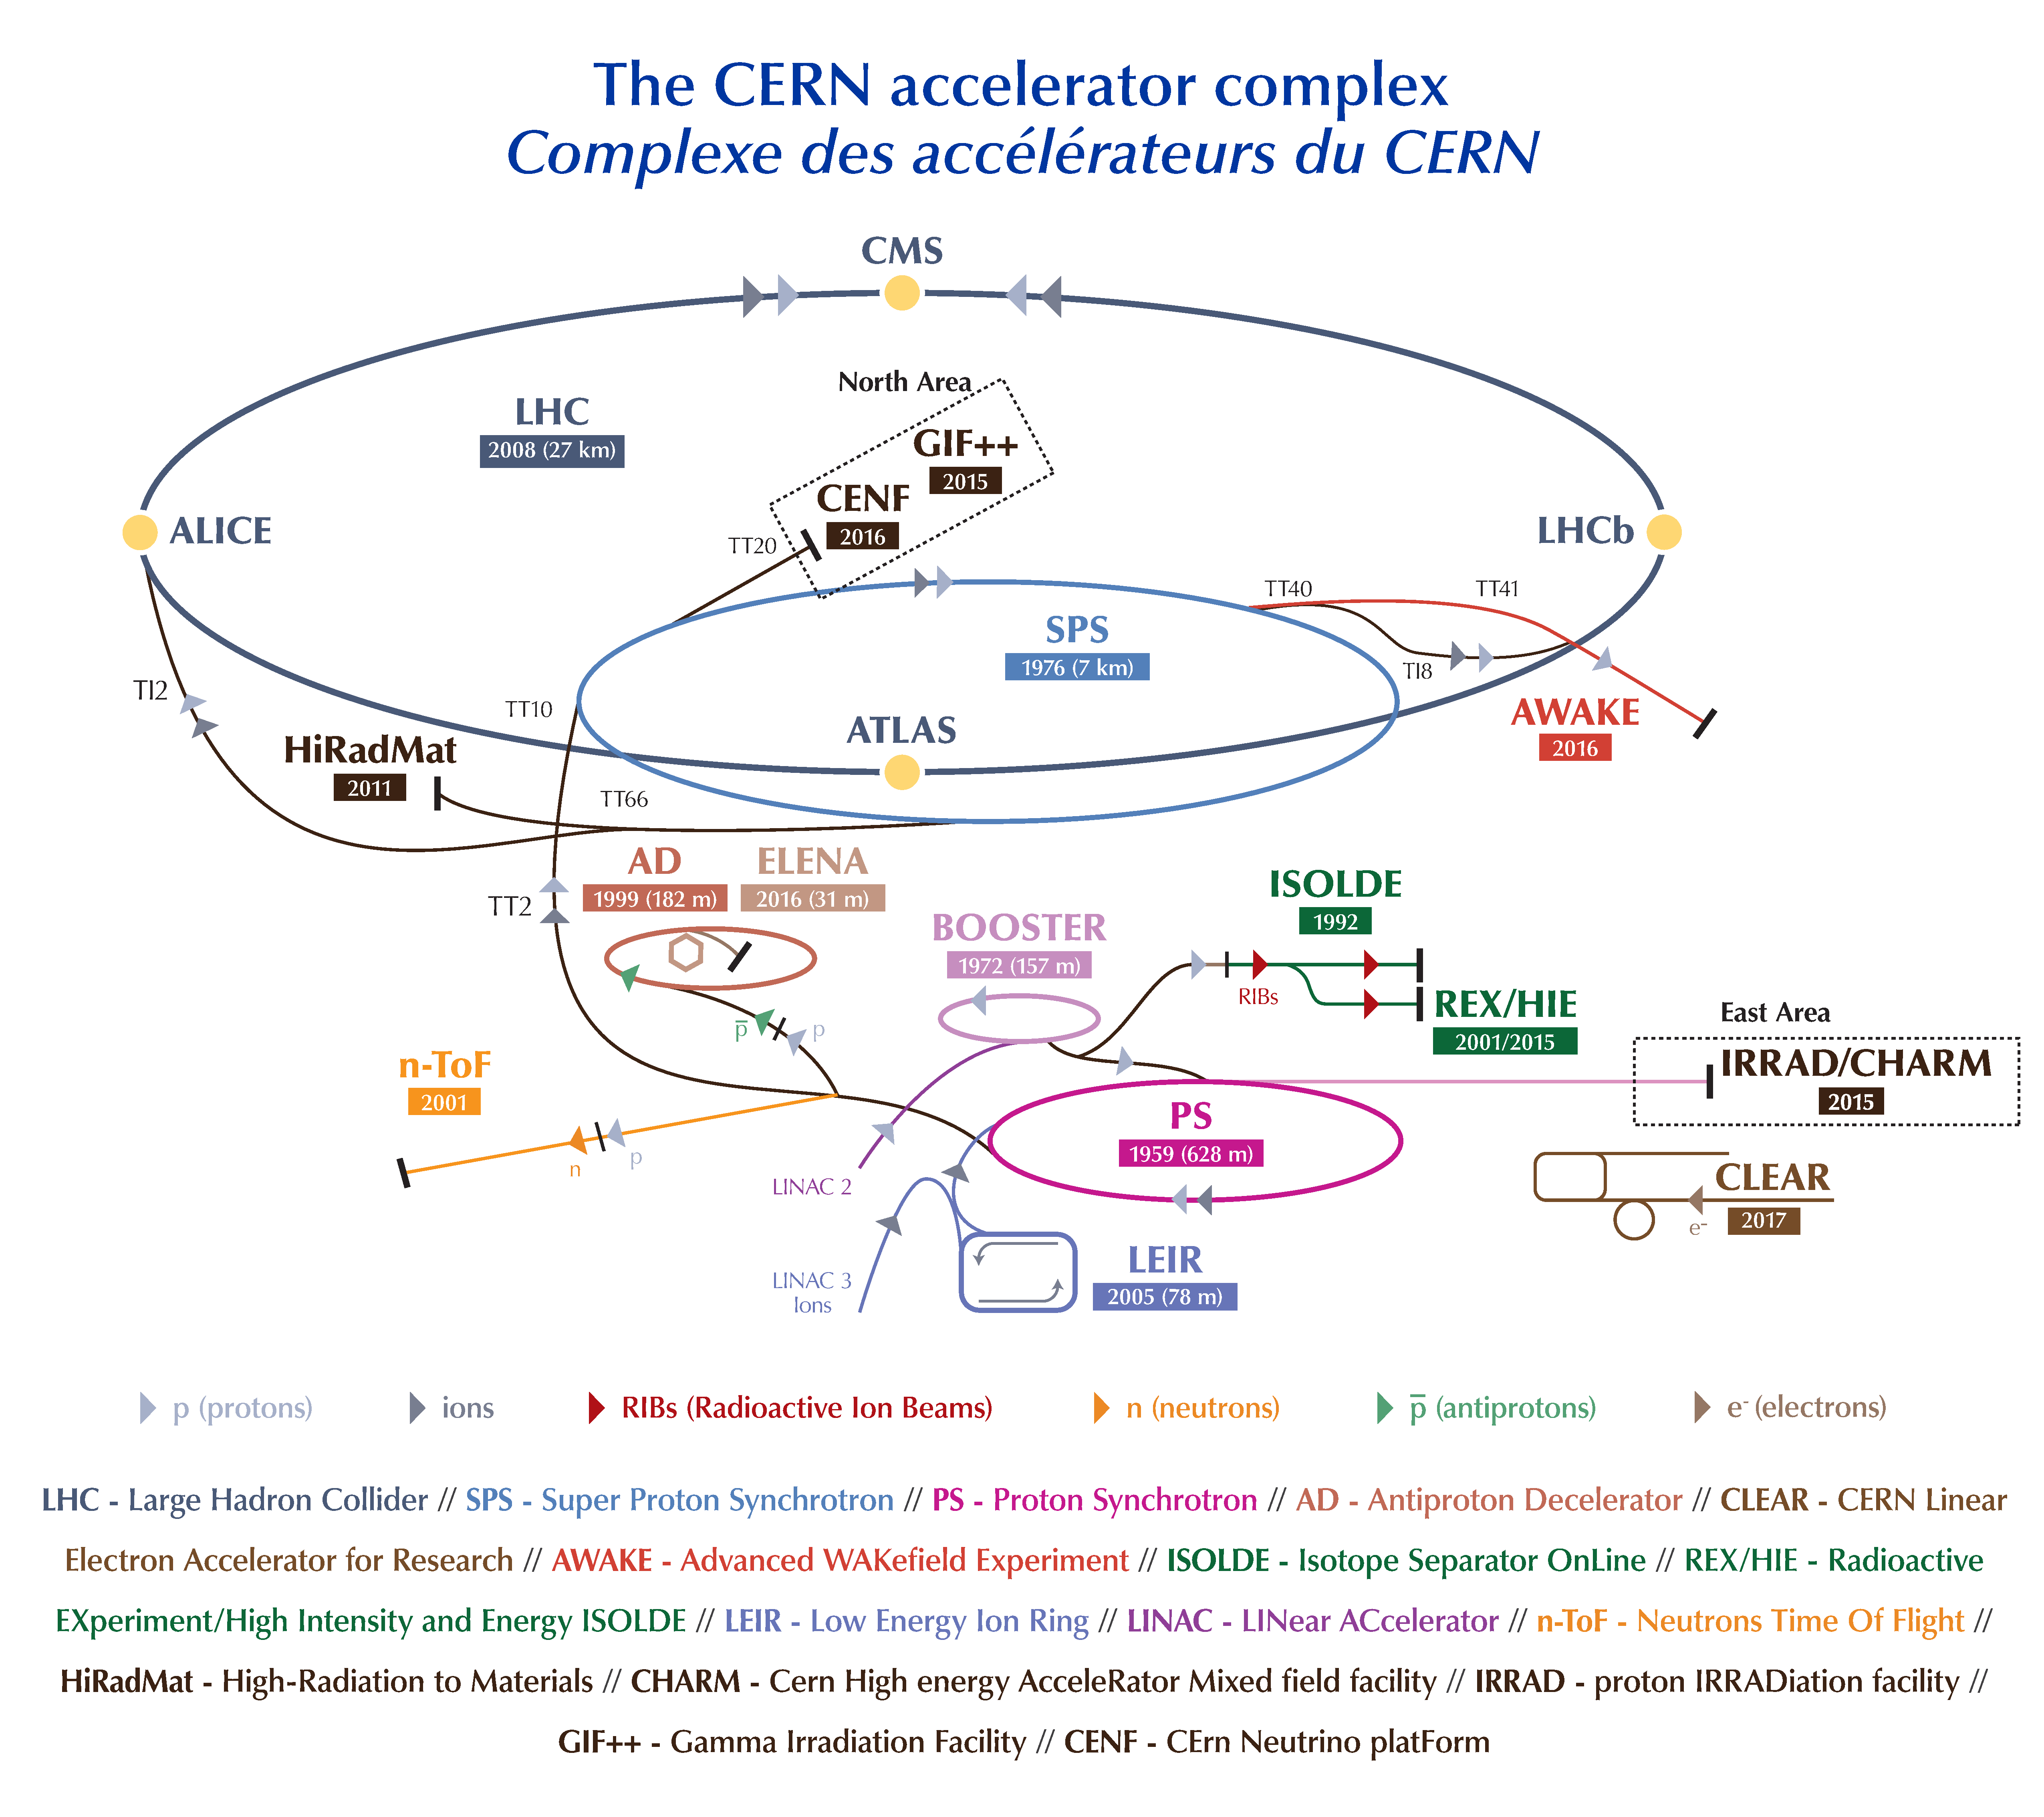
\includegraphics[width=0.65\textwidth]{Figs/CH4/LHC_ring.png}
    \caption[Schematic overview of the CERN accelerator complex.]{
    Schematic layout of the CERN accelerator complex, including the LHC ring and its main interaction regions~\cite{Mobs2018CERNAcceleratorComplex}.
    }
    \label{fig:lhc_layout}
\end{figure}

The LHC was proposed as the next major collider after LEP.
The first circulating beams were achieved in 2008, and the first physics run began in 2010.
The discovery of a new boson compatible with the Standard Model~(SM) Higgs boson by the ATLAS and CMS experiments in 2012 marked one of the central achievements of the LHC physics programme~\cite{ATLAS2012Higgs,CMS2012Higgs}.
Beyond Higgs-boson measurements and precision studies of SM processes, a major purpose of the LHC is to search for new particles and interactions beyond the SM.

The LHC collides protons at high centre-of-mass energies in order to extend the kinematic reach for the production of heavy particles.
For two proton beams with equal beam energy $E_{\mathrm{beam}}$, the proton--proton centre-of-mass energy is approximately $\sqrt{s}=2E_{\mathrm{beam}}$.
However, the hard-scattering process in a proton--proton~($pp$) collision occurs between partons, namely quarks and gluons, which carry only fractions of the proton momenta.
The partonic centre-of-mass energy therefore varies from event to event and is generally lower than the nominal $pp$ collision energy.
Increasing $\sqrt{s}$ consequently extends the accessible mass range for new heavy particles.

Another key machine parameter is the luminosity, which quantifies the collision rate per unit cross section.
For a process with cross section $\sigma$, the production rate is
\begin{align}
    R = \mathcal{L}\sigma,
    \label{eq:lhc_event_rate}
\end{align}
where $\mathcal{L}$ is the instantaneous luminosity.
For two Gaussian bunches colliding with frequency $f_{\mathrm{coll}}$, the luminosity can be expressed as~\cite{Herr2006Luminosity}
\begin{align}
    \mathcal{L}
    =
    f_{\mathrm{coll}}
    \frac{n_{1}n_{2}}
    {4\pi\sigma^{*}_{x}\sigma^{*}_{y}}
    \mathcal{F},
    \label{eq:lhc_luminosity_formula}
\end{align}
where $n_{1}$ and $n_{2}$ are the numbers of particles in the two colliding bunches, $\sigma^{*}_{x}$ and $\sigma^{*}_{y}$ are the RMS transverse beam sizes in the horizontal and vertical directions at the interaction point, and $\mathcal{F}$ is a geometrical reduction factor accounting for effects such as the crossing angle.
The integrated luminosity,
\begin{align}
    \mathcal{L}_{\mathrm{int}}
    =
    \int \mathcal{L}\,dt,
    \label{eq:lhc_integrated_luminosity}
\end{align}
determines the total expected number of produced events by $N=\sigma\mathcal{L}_{\mathrm{int}}$.
High instantaneous luminosity increases the event rate, while high integrated luminosity improves the sensitivity to rare processes with small production cross sections.

Four major experiments are installed around the LHC ring.
ATLAS, located at Point~1, and CMS, located at Point~5, are general-purpose detectors designed for a broad physics programme including Higgs-boson measurements, precision SM studies, and searches for new particles.
ALICE, located at Point~2, is optimised for heavy-ion physics and the study of strongly interacting matter at high energy density.
LHCb, located at Point~8, is designed for precision studies of heavy-flavour hadrons and flavour-changing processes~\cite{Evans2008LHC}.
The analysis presented in this thesis uses data recorded by the ATLAS detector.

The LHC physics programme is organised into run periods.
Run~1 took place from 2010 to 2012, with $pp$ collision data recorded at $\sqrt{s}=7~\TeV$ and $\sqrt{s}=8~\TeV$.
Run~2 took place from 2015 to 2018 at $\sqrt{s}=13~\TeV$.
After standard data-quality selections, the full ATLAS Run~2 $pp$ dataset corresponds to an integrated luminosity of $140.1\pm1.2~\ifb$, with a relative uncertainty of $0.83\%$~\cite{ATLASLumiRun2}.
Run~3 began in 2022 after the second long shutdown and operated at the higher centre-of-mass energy of $\sqrt{s}=13.6~\TeV$~\cite{ATLASRun3Starts}.
The Run~2 dataset is used for the leptoquark search presented in this thesis.

An important consequence of high-luminosity operation at the LHC is pile-up.
The proton beams are divided into bunches, and a bunch crossing occurs when bunches from the two beams pass through the interaction point.
Several $pp$ interactions can occur in a single bunch crossing.
The interaction corresponding to the hard-scattering process of interest is referred to as the hard-scatter interaction, while additional inelastic $pp$ interactions in the same bunch crossing constitute in-time pile-up.
Detector signals may also originate from interactions in neighbouring bunch crossings, depending on the detector response time. This contribution is referred to as out-of-time pile-up.

The mean number of inelastic $pp$ collision per bunch crossing is commonly denoted by $\mu$.
During Run~2, the nominal bunch spacing was $25~\mathrm{ns}$, corresponding to a maximum bunch-crossing frequency of $40~\mathrm{MHz}$.
Each of the bunch crossing over the full Run~2 period contains approximately $\langle\mu\rangle=34$~\cite{ATLASPileupJER2024}.

Pile-up has an important impact on event reconstruction.
It produce extra charged-particle tracks, calorimeter energy deposits, and reconstructed jets.
They can affect the reconstruction of the primary vertex, jet energies, hadronically decaying $\tau$-leptons, flavour-tagged jets, and missing transverse momentum. Pile-up effects must be therefore modelled in simulated samples and mitigated through dedicated reconstruction and calibration procedures.


\section{ATLAS experiment}
\label{sec:atlas_experiment}

\subsection{Overview}
\label{subsec:atlas_overview}

ATLAS, which stands for A Toroidal LHC ApparatuS, is a detector located at Point~1 of the Large Hadron Collider.
It was designed to exploit the full physics potential of the LHC, including precision measurements of SM processes, studies of the Higgs boson, and searches for new physics beyond the SM.
The detector surrounds the nominal interaction point and provides nearly full solid-angle coverage, allowing the reconstruction of a wide range of final-state particles produced in proton--proton collisions.

The ATLAS detector is approximately $44~\mathrm{m}$ long, $25~\mathrm{m}$ in diameter, and has a total weight of about $7000~\mathrm{tonnes}$~\cite{ATLASDetector2008}.
It has a cylindrical, forward--backward symmetric layout centred on the interaction point.
A schematic view of the detector is shown in Figure~\ref{fig:ATLAS_view}.

\begin{figure}[htbp]
    \centering
    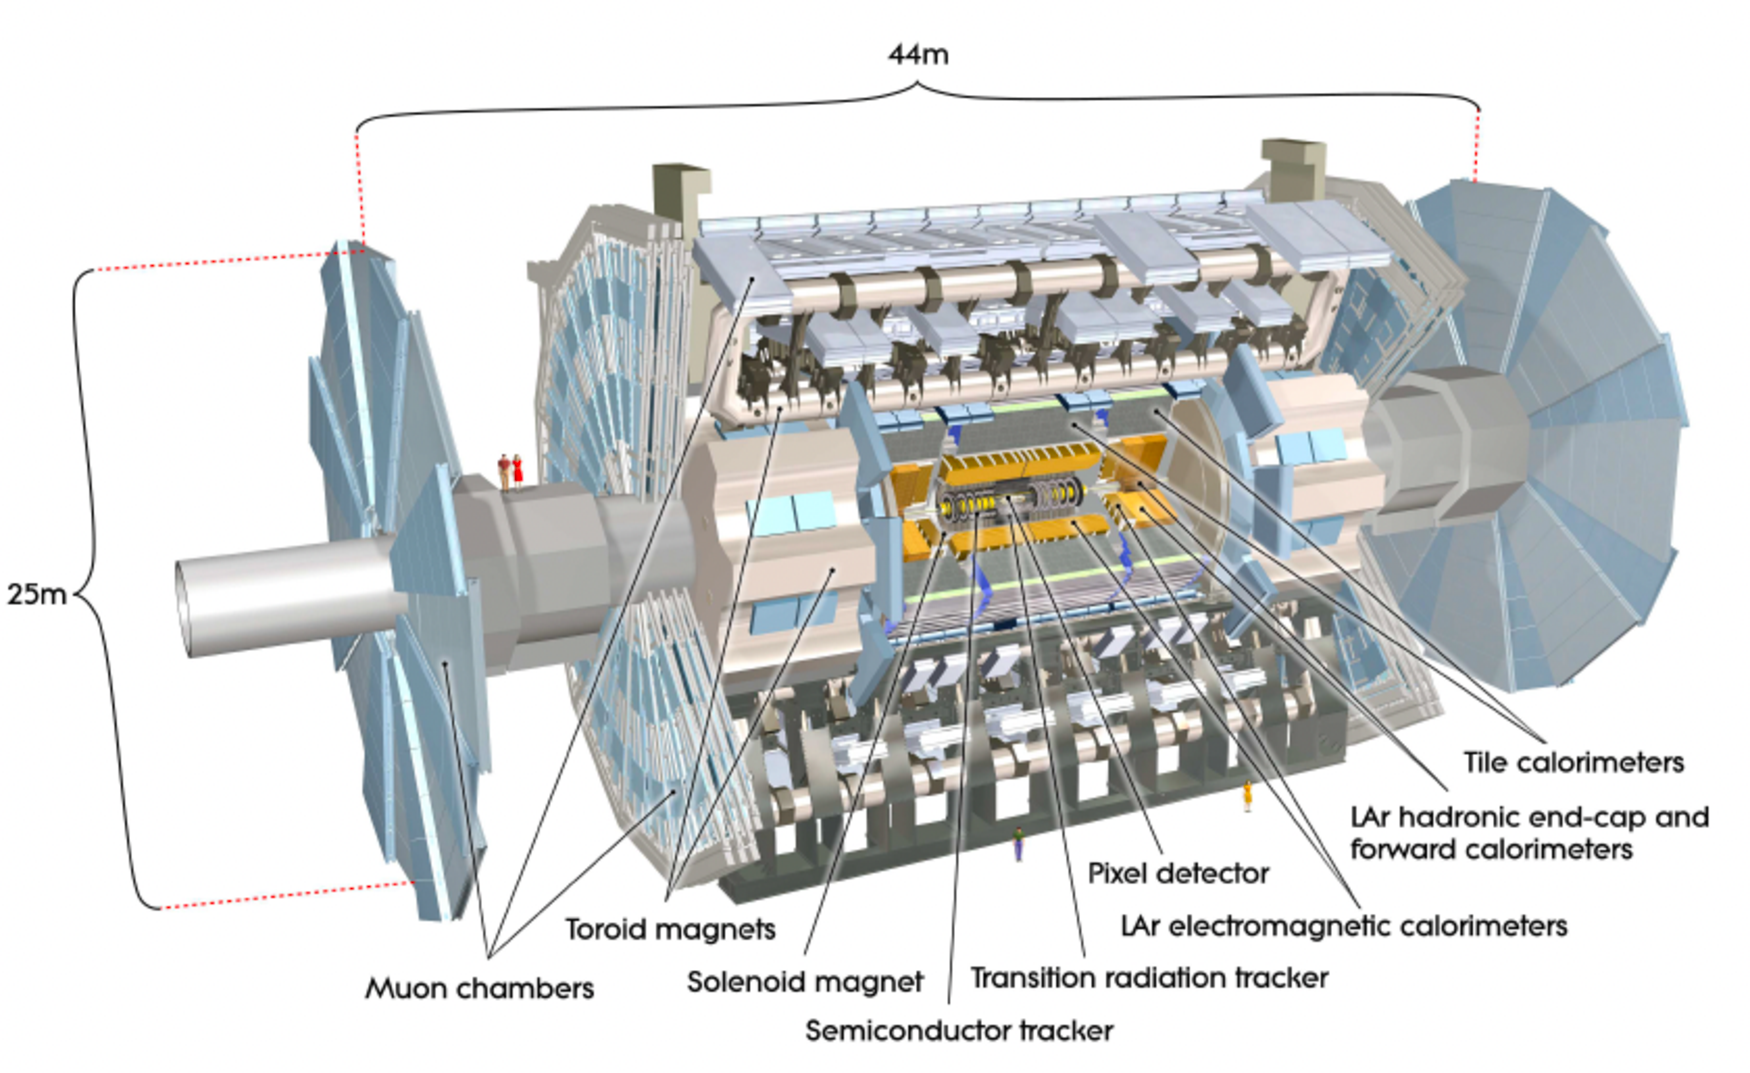
\includegraphics[width=0.9\linewidth]{Figs/CH4/ATLAS_slide.pdf}
    \caption[The schematic view of the ATLAS detector and the subdetector systems]{
    Schematic view of the ATLAS detector and its subdetector systems~\cite{ATLASDetector2008}.
    }
    \label{fig:ATLAS_view}
\end{figure}

Starting from the beam line and moving outwards, the main detector systems are the Inner Detector~(ID), the calorimeters, and the Muon Spectrometer~(MS)~\cite{ATLASDetector2008}:
\begin{itemize}
    \item \textbf{\textit{Inner Detector (ID)}} is immersed in a $2~\mathrm{T}$ axial magnetic field provided by a thin superconducting solenoid and is used to reconstruct charged-particle trajectories close to the interaction point.
    \item \textbf{\textit{Calorimeters}} surround the ID and measure the energies of electrons, photons, hadrons, hadronically decaying $\tau$-leptons, and jets.
    \item \textbf{\textit{Muon Spectrometer (MS)}} forms the outermost major detector system and measures muons in the magnetic field generated by large superconducting toroids.
\end{itemize}
The magnetic fields provided by the solenoid and toroids allow the momentum and charge of charged particles to be determined from the curvature of their trajectories.
The trigger and data acquisition system selects potentially interesting events from the high LHC bunch-crossing rate for permanent storage and offline reconstruction.

The detector configuration described in this chapter corresponds primarily to Run~2.
Several detector and trigger upgrades were installed for Run~3 to cope with higher luminosity conditions, but these upgrades are not used in the analysis presented in this thesis~\cite{ATLASRun3Detector}.


\subsection{Coordinate system}
\label{subsec:atlas_coordinate_system}

ATLAS uses a right-handed coordinate system centred at the nominal interaction point.
The $z$-axis is defined along the beam direction, the $x$-axis points from the interaction point towards the centre of the LHC ring, and the $y$-axis points upwards~\cite{ATLASDetector2008}.
Cylindrical coordinates $(r,\phi)$ are used in the plane transverse to the beam, where $r$ is the distance from the beam axis and $\phi$ is the azimuthal angle around the $z$-axis.

The polar angle $\theta$ is measured with respect to the positive $z$-axis.
The pseudorapidity $\eta$ is defined as
\begin{align}
    \eta
    =
    -\ln \tan \left( \frac{\theta}{2} \right).
    \label{eq:pseudorapidity}
\end{align}
The transverse momentum is defined as $p_{\mathrm{T}}=p\sin\theta$, and the transverse energy is defined similarly.
The angular separation between two reconstructed objects is commonly expressed as
\begin{align}
    \Delta R
    =
    \sqrt{
        \left(\Delta \eta \right)^{2}
        +
        \left(\Delta \phi \right)^{2}
    }.
    \label{eq:delta_r}
\end{align}
These quantities are used throughout this thesis to describe object kinematics, angular separations, overlap removal, and event selections.
Figure~\ref{fig:coordinate_system} illustrates the coordinate system used in ATLAS.

\begin{figure}[htbp]
    \centering
    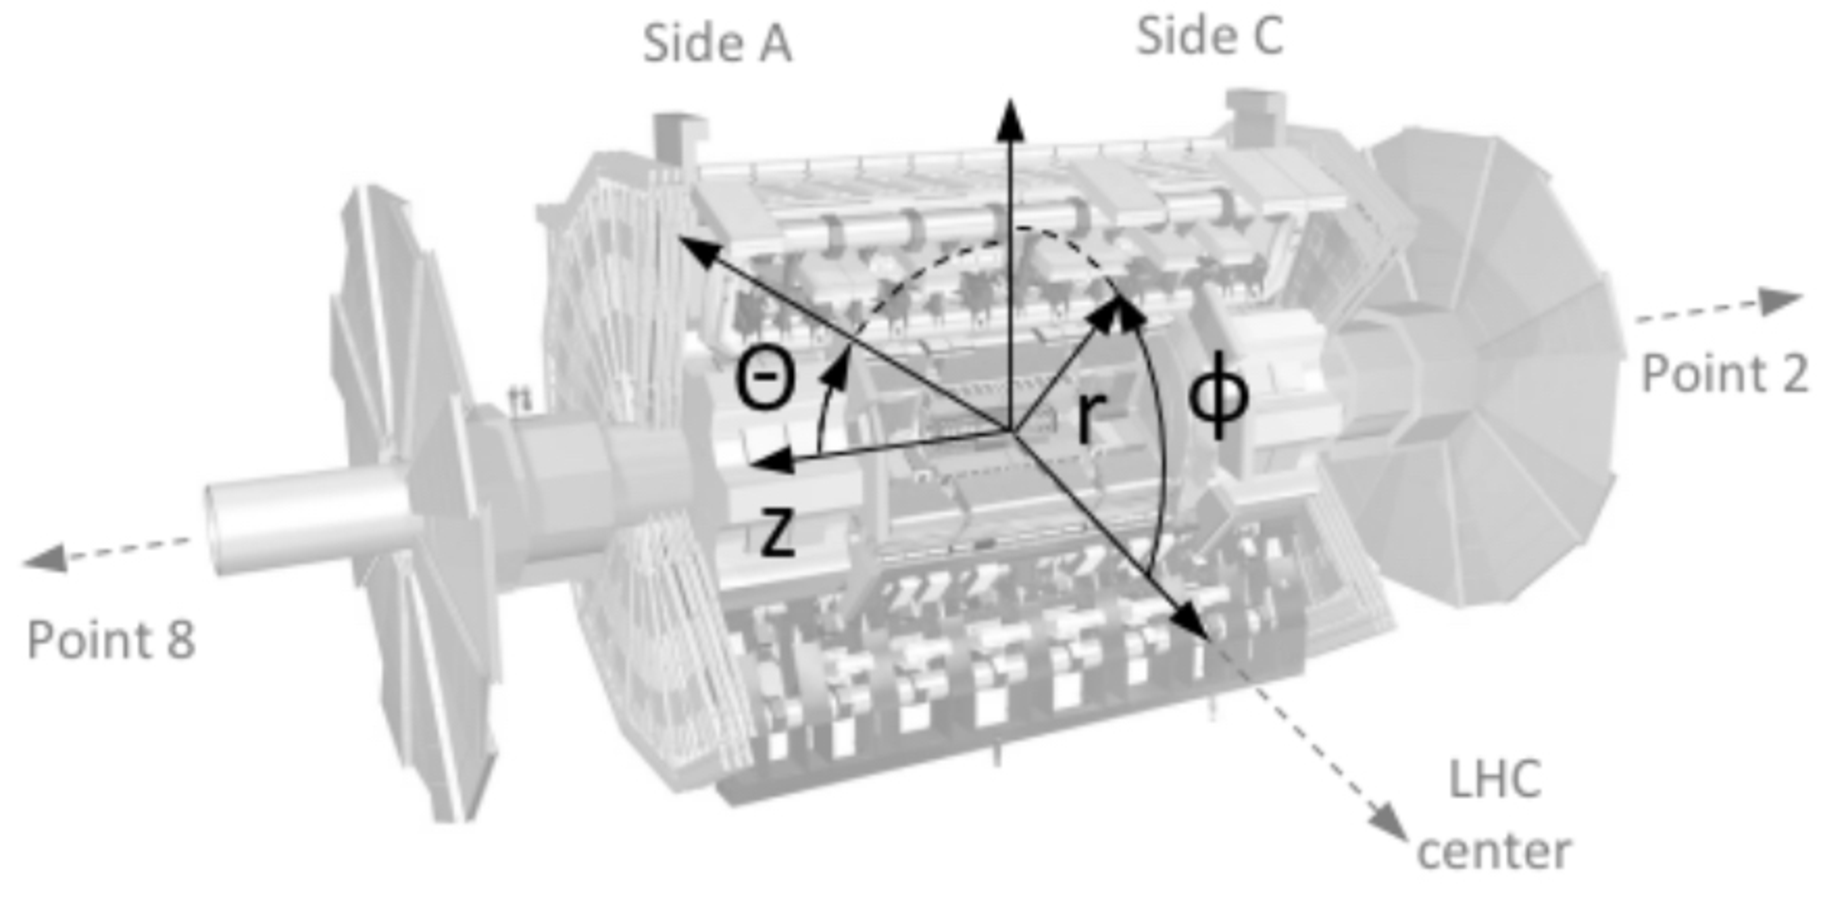
\includegraphics[width=0.7\linewidth]{Figs/CH4/coordinate system.pdf}
    \caption[The coordinate system used in ATLAS]{
    The coordinate system used in ATLAS~\cite{kuger2017signal}.
    }
    \label{fig:coordinate_system}
\end{figure}


\subsection{Magnet system}
\label{subsec:atlas_magnet_system}

The ATLAS magnet system consists of four large superconducting magnets: a central solenoid, one barrel toroid, and two end-cap toroids, as shown in Figure~\ref{fig:atlas_magnet_system}.
The central solenoid surrounds the Inner Detector with a length of approximately $5.3~\mathrm{m}$ and provides an axial magnetic field of $2~\mathrm{T}$ for charged-particle momentum measurements in the tracking system.
The solenoid is designed to minimise the amount of inactive material in front of the electromagnetic calorimeter.

The toroid system provides magnetic fields of approximately $0.5~\mathrm{T}$ and $1~\mathrm{T}$ in the barrel and end-cap regions of the Muon Spectrometer, respectively.
The barrel toroid surrounds the calorimeter system in the central region, while the two end-cap toroids provide bending power in the forward regions.
The toroidal field bends muon trajectories, allowing their momenta to be measured using the precision tracking chambers of the MS.
The air-core design of the toroids reduces multiple scattering and helps preserve the momentum resolution for high-$\pt$ muons~\cite{ATLASDetector2008}.
The combination of the solenoid and toroid systems allows charged-particle momenta to be measured independently in the ID and, for muons, in the MS.

\begin{figure}[htbp]
    \centering
    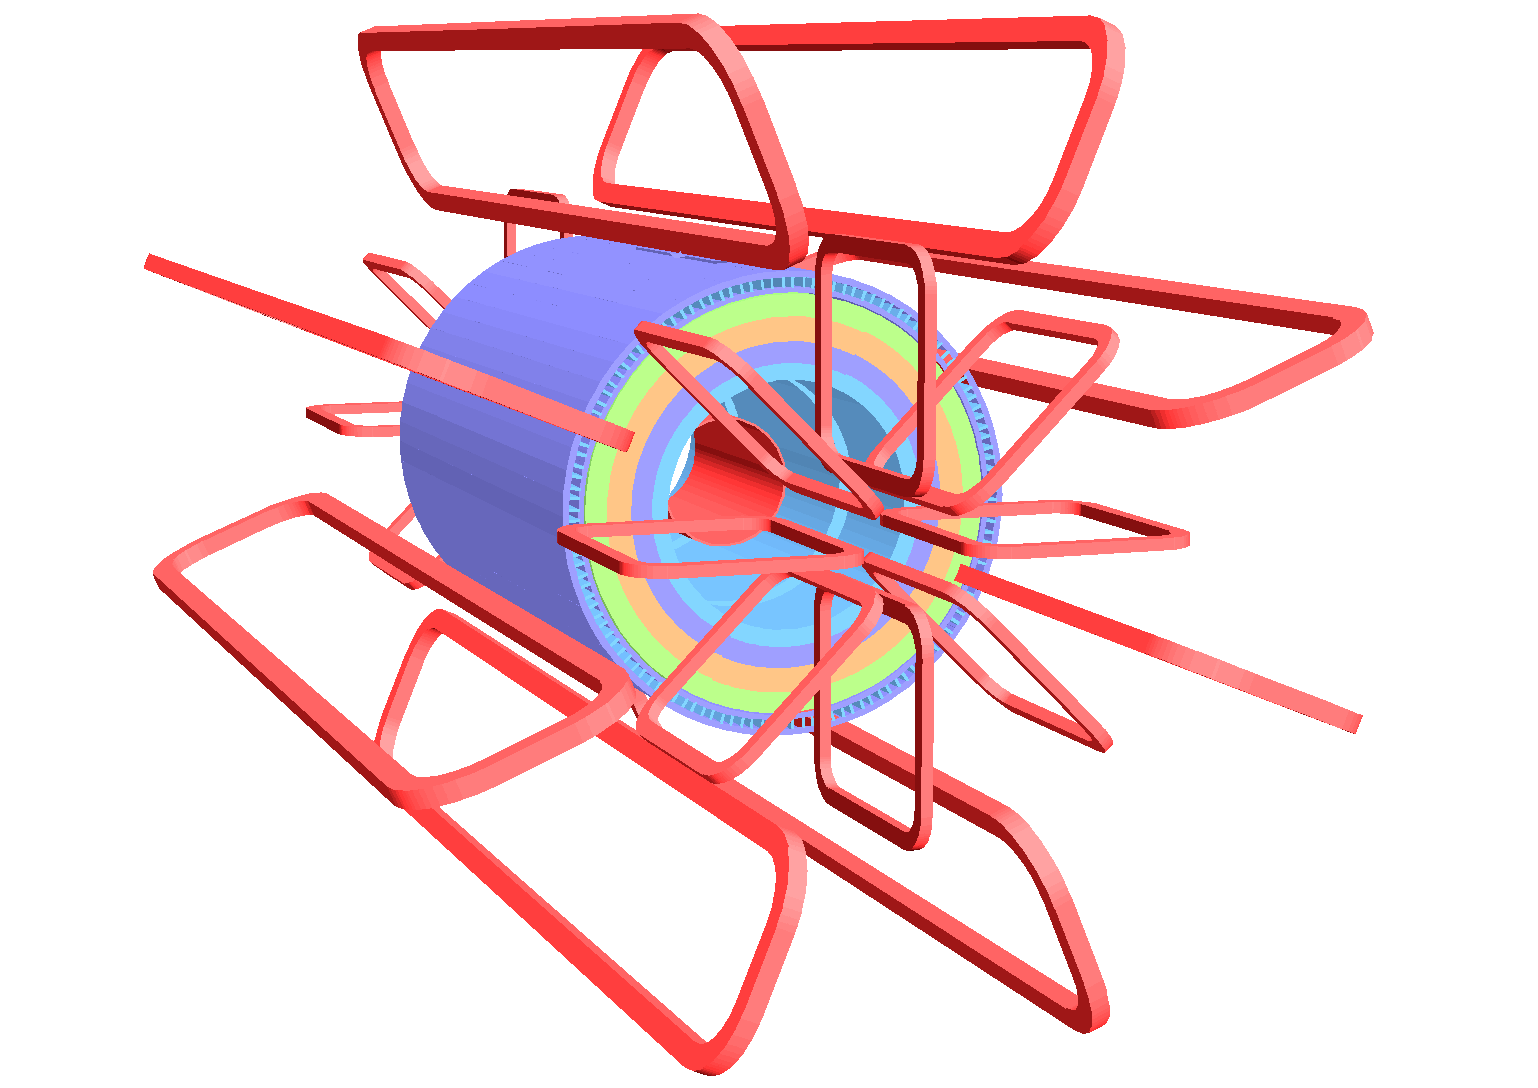
\includegraphics[width=0.65\textwidth]{Figs/CH4/ATLAS_magnet.pdf}
    \caption[ATLAS magnet system]{
    Layout of the ATLAS superconducting magnet system, including the central solenoid, barrel toroid, and end-cap toroids~\cite{ATLASDetector2008}.
    }
    \label{fig:atlas_magnet_system}
\end{figure}


\subsection{Inner Detector}
\label{subsec:atlas_inner_detector}

The Inner Detector~(ID) is the innermost tracking system of ATLAS.
It is immersed in the $2~\mathrm{T}$ magnetic field of the central solenoid and provides tracking for charged particles within $|\eta|<2.5$~\cite{ATLASDetector2008}.
During Run~2, it consisted of the pixel detector, the Semiconductor Tracker~(SCT), and the Transition Radiation Tracker~(TRT). The Insertable B-Layer~(IBL) is installed before Run~2 as the innermost pixel layer~\cite{ATLASIBL2018}.
Figure~\ref{fig:atlas_inner_detector} shows a transverse view of the Inner Detector.

\begin{itemize}
    \item \textbf{\textit{Insertable B-Layer~(IBL) and Pixel detector\quad}}

    The pixel detector provides high-granularity measurements close to the beam line.
    Its precise spatial resolution is essential for reconstructing tracks near the interaction point and for identifying displaced vertices from the decays of long-lived particles such as $b$- and $c$-hadrons.
    The IBL further improves the impact-parameter resolution and enhances the robustness of tracking and flavour tagging under high pile-up conditions.

    \item \textbf{\textit{Semiconductor Tracker~(SCT)\quad}}

    The SCT surrounds the pixel detector and forms the intermediate precision-tracking system of the ID.
    It is a silicon microstrip detector covering $|\eta|<2.5$, consisting of four cylindrical barrel layers and two end-caps with nine disks on each side.
    Each module contains silicon strip sensors arranged back-to-back with a small stereo angle, allowing two-dimensional position information to be reconstructed.
    The SCT typically provides four space-point measurements per track, improving pattern recognition, momentum reconstruction, and vertex reconstruction when combined with the high-granularity pixel measurements.

    \item \textbf{\textit{Transition Radiation Tracker~(TRT)\quad}}

    The TRT is the outermost tracking subsystem of the ID and provides tracking information at larger radii, covering approximately $|\eta|<2.0$~\cite{ATLASDetector2008}.
    It is based on thin straw-tube drift chambers, which provide a large number of measurements along the trajectory of each charged particle.
    Although the spatial precision of each TRT hit is lower than that of the silicon detectors, the large number of straw hits and the longer lever arm improve the momentum measurement and help stabilise track reconstruction.
\end{itemize}

Together, these subsystems provide the tracking information needed in ATLAS.

\begin{figure}[htbp]
    \centering
    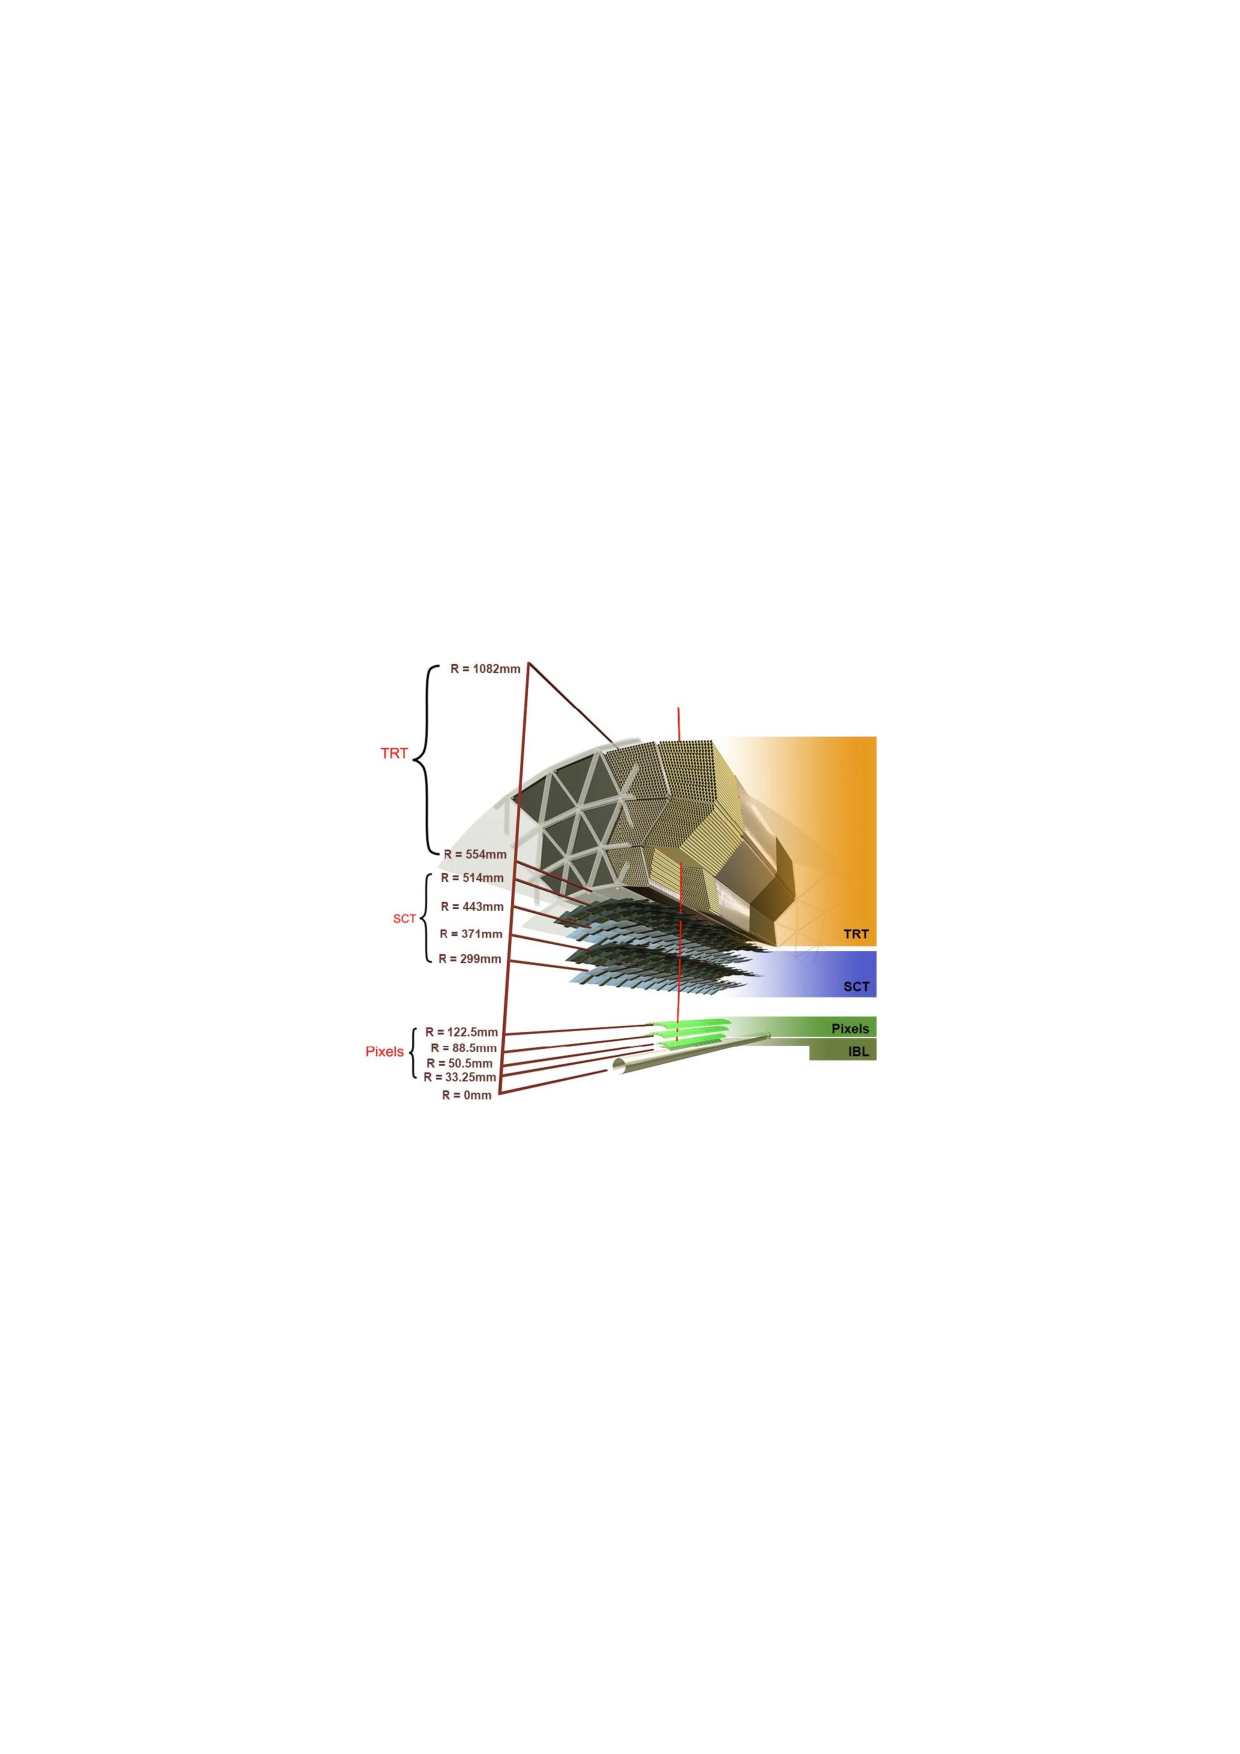
\includegraphics[width=0.65\textwidth]{Figs/CH4/ATLAS_IBL.pdf}
    \caption[ATLAS Inner Detector]{
    Transverse view of the ATLAS Inner Detector, showing the IBL, pixel detector, SCT, and TRT subsystems~\cite{ATLASIBL2018}.
    }
    \label{fig:atlas_inner_detector}
\end{figure}


\subsection{Calorimeter}
\label{subsec:atlas_calorimeter}

The ATLAS calorimeter system surrounds the Inner Detector and measures the energies and directions of particles.
It consists of electromagnetic~(EM) and hadronic calorimeters, as shown in Figure~\ref{fig:atlas_calorimeter}. Specifically, it provides measurements of charged particles, photons and jets, and covers the region up to $|\eta|<4.9$. It also provides the shower information to the Level-1 trigger system.


\begin{figure}[htbp]
    \centering
    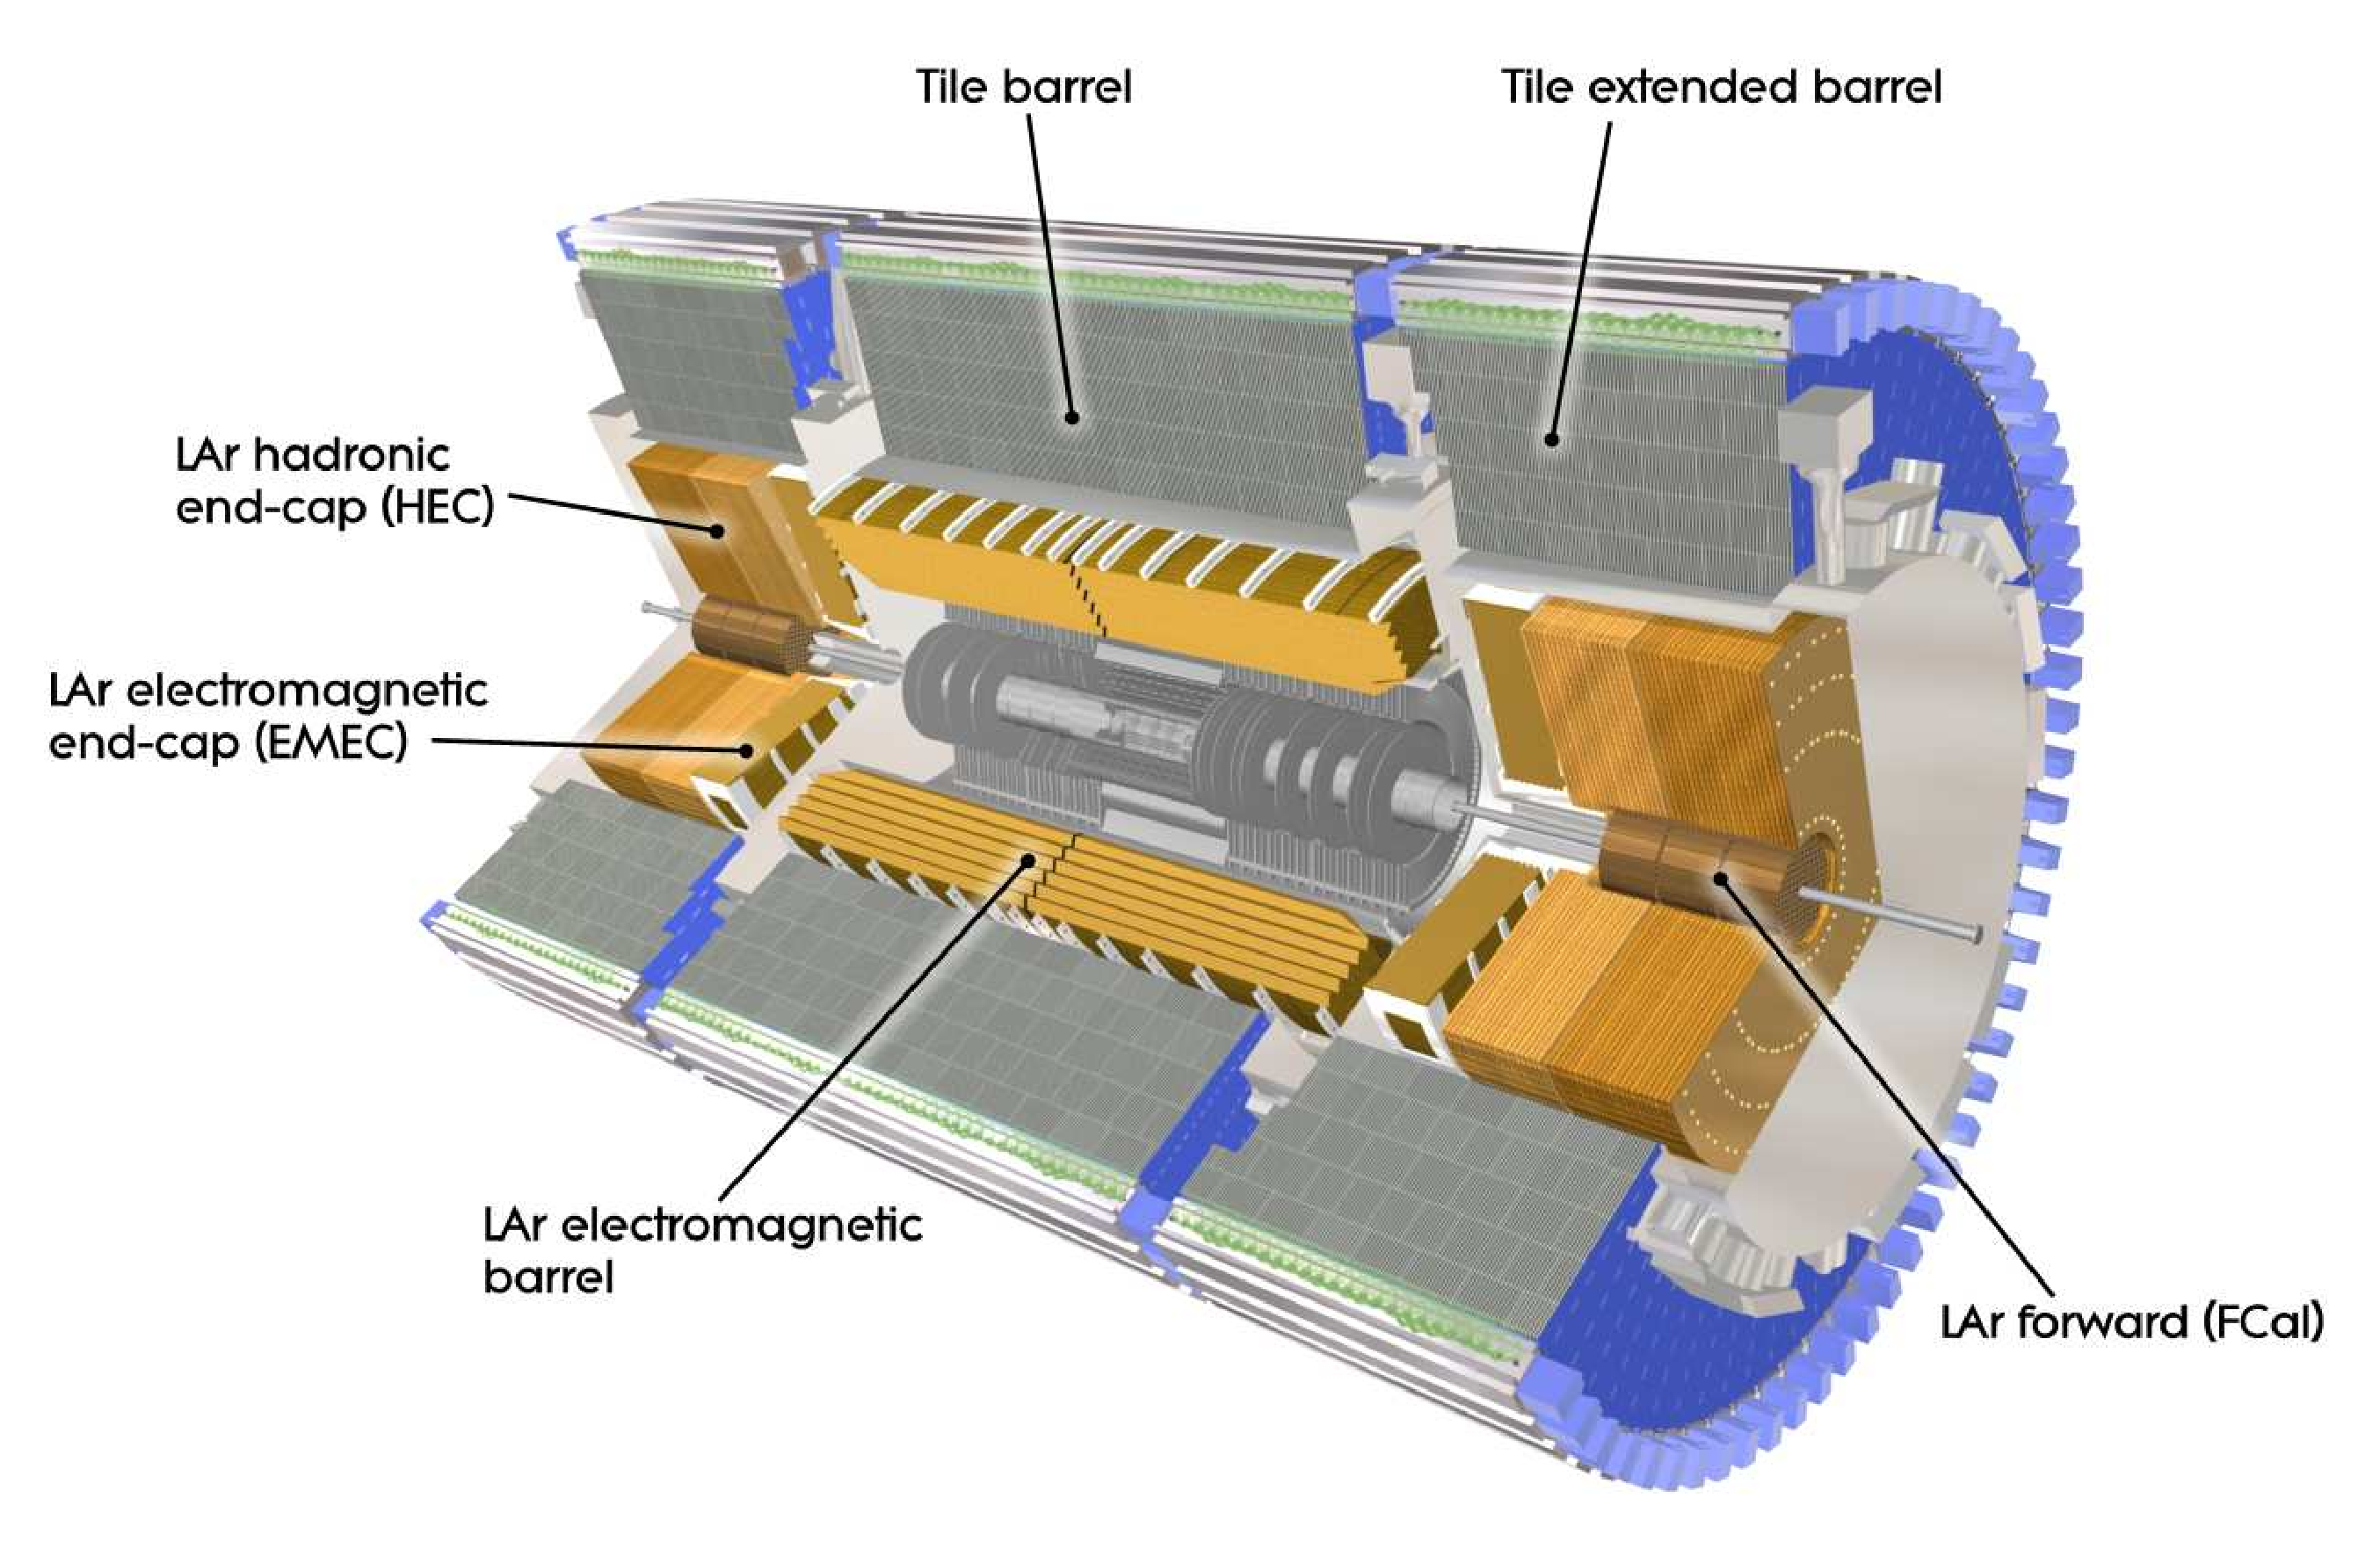
\includegraphics[width=0.85\textwidth]{Figs/CH4/LAr_calo_view.pdf}
    \caption[ATLAS calorimeter system]{
    Schematic view of the ATLAS calorimeter system~\cite{ATLASDetector2008}.
    }
    \label{fig:atlas_calorimeter}
\end{figure}

\begin{itemize}
    \item \textbf{\textit{Electromagnetic (EM) calorimeter\quad}}

    The EM calorimeter uses liquid argon~(LAr) as the active medium and lead absorbers arranged in an accordion geometry, as shown in Figure~\ref{fig:LAr_module}.
    The accordion geometry provides continuous azimuthal coverage and fine segmentation of electromagnetic showers~\cite{ATLASDetector2008}.
    The EM calorimeter is divided into a barrel section covering $|\eta|<1.475$ and two end-cap sections covering $1.375<|\eta|<3.2$.
    It is used to reconstruct and identify electrons and photons and also contributes to the reconstruction of hadronically decaying $\tau$-leptons, particularly through the measurement of electromagnetic energy deposits from neutral-pion decays, which don't leave the charged-particle tracks in the ID.

    The EM calorimeter consists of a presampler followed by three longitudinal sampling layers, each segmented into readout cells, as illustrated in Figure~\ref{fig:LAr_cells}.
    The presampler is installed for $|\eta|<1.8$ and is used to correct for energy lost in material upstream of the calorimeter.
    The first sampling layer has fine segmentation in $\eta$, which is useful for resolving the transverse shape of electromagnetic showers, while the middle layer collects the largest fraction of the shower energy.
    The back layer provides an additional measurement of the longitudinal shower development.

    The energy resolution of the electromagnetic calorimeter can be parameterised as
    \begin{align}
        \frac{\sigma_E}{E}
        =
        \frac{a}{\sqrt{E}}
        \oplus b
        \oplus \frac{c}{E},
        \label{eq:resolution}
    \end{align}
    where $a$ is the intrinsic sampling term, $b$ is the constant term, and $c$ represents the contribution from electronic and pile-up noise~\cite{readout}.

\begin{figure}[htbp]
    \centering
    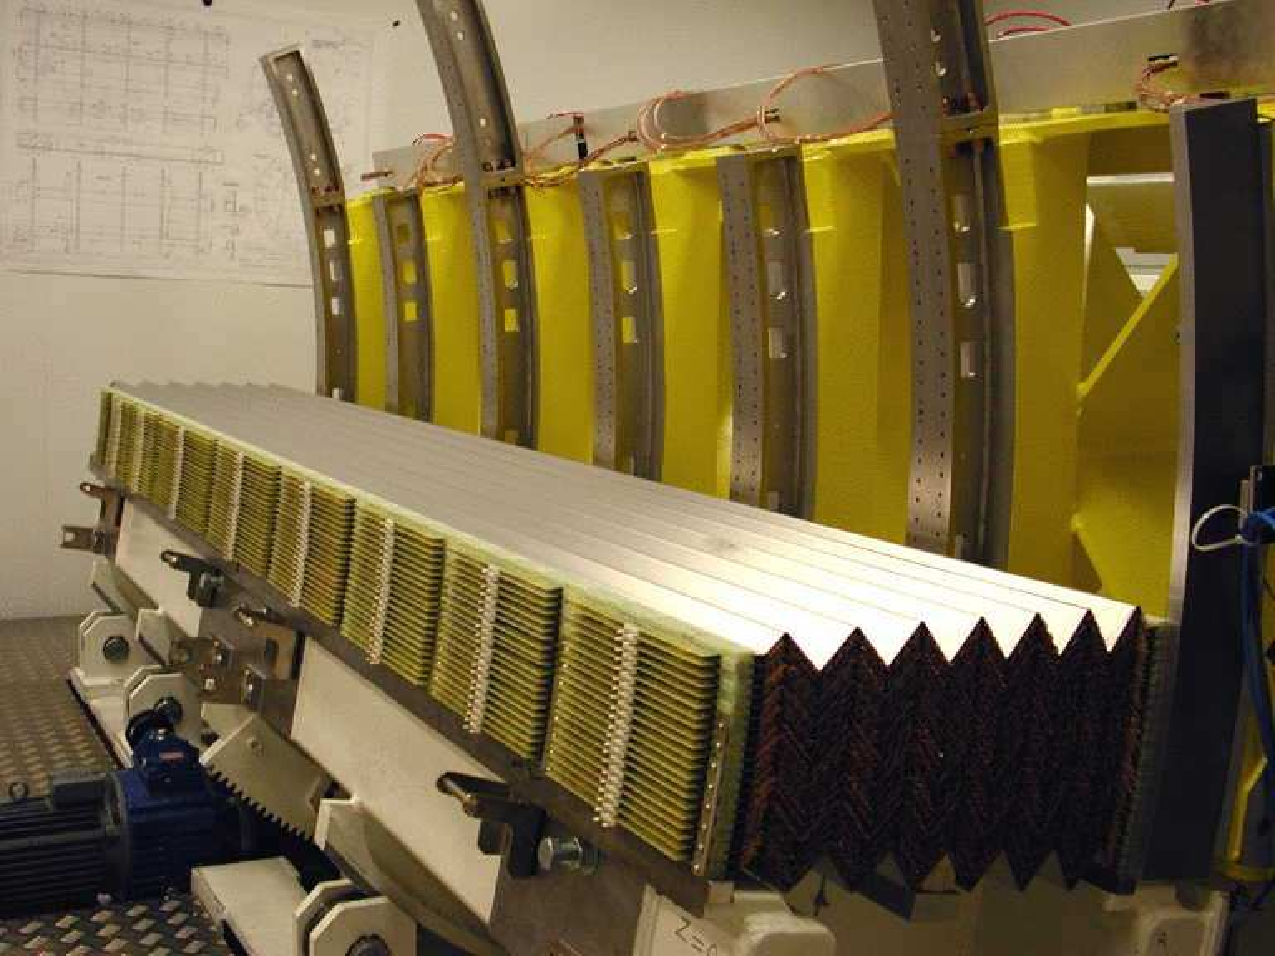
\includegraphics[width=0.40\linewidth]{Figs/CH4/lar_barrel.pdf}
    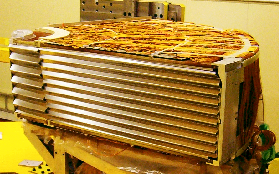
\includegraphics[width=0.48\linewidth]{Figs/CH4/LAr_EndCap.png}
    \caption[Photograph of EM barrel and end-cap LAr modules]{
    Photograph of the EM barrel (left) and end-cap (right) LAr modules.
    The accordion absorber structure is visible~\cite{ATLASDetector2008}.
    }
    \label{fig:LAr_module}
\end{figure}

\begin{figure}[htbp]
    \centering
    \includegraphics[width=0.5\linewidth]{Figs/CH4/LAr_cells.pdf}
    \caption[A cut-away view of an LAr electromagnetic calorimeter module]{
    Cut-away view of an ATLAS LAr electromagnetic calorimeter module, showing the longitudinal sampling layers and the segmentation of the readout cells~\cite{ATLASDetector2008}.
    }
    \label{fig:LAr_cells}
\end{figure}

    \item \textbf{\textit{Hadronic calorimeter\quad}}

    The hadronic calorimeter uses different structure for different $\eta$ regions.
    In the region of $|\eta|<1.7$, the Tile Calorimeter uses steel absorbers and scintillating tiles as the active medium.
    It measures the energies of hadrons and jets.
    In the end-cap and forward regions, liquid-argon calorimeters are used.
    The hadronic end-cap calorimeter consists of two wheels per end-cap, covers the range $1.5<|\eta|<3.2$, and uses copper absorbers.
    The forward calorimeter extends the coverage to $3.1<|\eta|<4.9$ and uses dense absorber materials suitable for the high-radiation environment close to the beam line~\cite{ATLASDetector2008}.
\end{itemize}


\subsection{Muon Spectrometer}
\label{subsec:atlas_muon_spectrometer}

The Muon Spectrometer~(MS) forms the outermost major detector system of ATLAS.
It is embedded in the magnetic field produced by the barrel and end-cap air-core toroid magnets.
The bending of muon trajectories in this field is measured by precision chambers, and the track sagitta is used to determine the muon momentum.
The MS provides precision muon measurements in the range $|\eta|<2.7$, while the dedicated muon trigger chambers cover the region up to approximately $|\eta|<2.4$~\cite{ATLASDetector2008}.

During Run~2, the MS consisted of Monitored Drift Tubes~(MDTs), Cathode Strip Chambers~(CSCs), Resistive Plate Chambers~(RPCs) and Thin Gap Chambers~(TGCs)~\cite{ATLASDetector2008}.
A view of these chambers is shown in Figure~\ref{fig:atlas_muon_spectrometer}.

\begin{itemize}
    \item \textbf{\textit{Monitored Drift Tubes~(MDTs)\quad}}

    The MDT chambers provide precision tracking over most of the MS acceptance.
    They consist of aluminium drift tubes with a diameter of about $30~\mathrm{mm}$, each containing a central sense wire.
    A muon crossing a tube ionises the gas, and the drift time of the electrons to the wire is measured to determine the track position.
    Several tube layers are grouped into chamber stations, providing precise measurements in the bending plane of the toroidal magnetic field.
    MDT chambers are used over most of the region $|\eta|<2.7$, except for the innermost forward stations at $2.0<|\eta|<2.7$, where CSCs are used.

    \item \textbf{\textit{Cathode Strip Chambers~(CSCs)\quad}}

    The CSCs are multi-wire proportional chambers used in the innermost forward muon stations, where the particle rates are highest.
    They cover approximately $2.0<|\eta|<2.7$ and provide precision measurements in the forward region~\cite{ATLASDetector2008}.
    Their small drift distance and segmented cathode-strip readout allow them to operate efficiently in the high-rate environment close to the beam line.

    \item \textbf{\textit{Resistive Plate Chambers~(RPCs)\quad}}

    The RPCs provide fast muon trigger information in the barrel region, covering approximately $|\eta|<1.05$~\cite{ATLASDetector2008}.
    They are gaseous parallel-plate detectors operated in avalanche mode.
    Their fast time response allows the bunch crossing associated with a muon candidate to be identified and provides the Level-1 muon trigger in the barrel.
    The RPCs also provide coordinate measurements complementary to the precision MDT chambers.

    \item \textbf{\textit{Thin Gap Chambers~(TGCs)\quad}}

    The TGCs are multi-wire proportional chambers designed to provide fast signals for the Level-1 trigger.
    They extend to approximately $|\eta|<2.7$ and provide trigger coverage in the end-cap region up to $|\eta|<2.4$~\cite{ATLASDetector2008}.
    The TGC system identifies high-$p_{\mathrm{T}}$ muon candidates and assigns them to the correct bunch crossing.
    It also provides a second coordinate measurement, complementing the precision tracking information from MDTs and CSCs.
\end{itemize}

\begin{figure}[htbp]
    \centering
    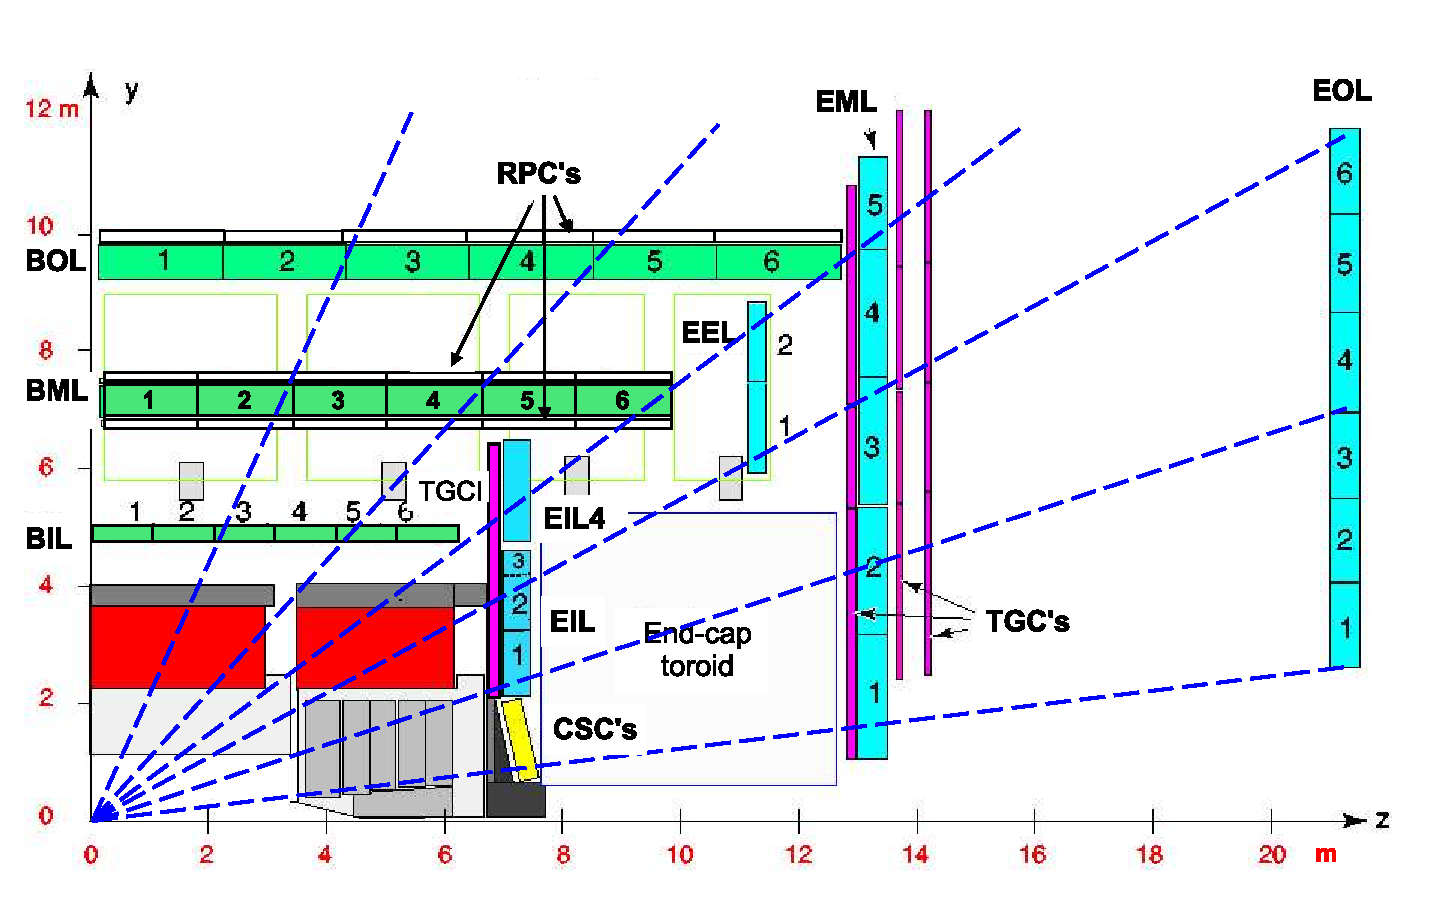
\includegraphics[width=0.85\textwidth]{Figs/CH4/ATLAS_MS.pdf}
    \caption[ATLAS Muon Spectrometer]{
    Cross-section of the ATLAS Muon Spectrometer, showing the barrel and end-cap muon chambers.
    The green and cyan chambers represent the MDT system, while the dashed lines indicate infinite-momentum muon trajectories~\cite{ATLASDetector2008}.
    }
    \label{fig:atlas_muon_spectrometer}
\end{figure}

During the second long shutdown, the innermost end-cap muon stations were replaced by the New Small Wheels~(NSWs) for Run~3 operation.
This upgrade was introduced to maintain good muon trigger and reconstruction performance under higher luminosity and pile-up conditions.
The NSW detectors are therefore not relevant to the Run~2 dataset analysed in this thesis.


\subsection{Data Acquisition and Trigger System}
\label{subsec:atlas_trigger_daq}

At the LHC, proton bunches can cross at a rate of up to $40~\mathrm{MHz}$ for a bunch spacing of $25~\mathrm{ns}$.
This rate is far above the available detector readout and permanent-storage bandwidth.
The ATLAS trigger and data acquisition~(TDAQ) system is therefore designed to select potentially interesting events online and reduce the event rate to a manageable level.
ATLAS uses a two-level trigger system consisting of a hardware-based Level-1~(L1) trigger and a software-based High-Level Trigger~(HLT)~\cite{ATLASTriggerRun2}.

\subsubsection*{Level-1 (L1) trigger}

The L1 trigger is the first stage of the ATLAS online event selection.
It is implemented in custom hardware and uses reduced-granularity detector information to make a fast decision with a latency of approximately $2.5~\mu\mathrm{s}$.
It reduces the input rate from up to $40~\mathrm{MHz}$ to at most $100~\mathrm{kHz}$~\cite{ATLASTriggerRun2}.
The L1 trigger was based on information from the calorimeter and muon trigger systems, together with topological selections applied to L1 trigger objects.
A schematic overview of the Run~2 TDAQ system is shown in Figure~\ref{fig:atlas_tdaq}.

\begin{figure}[htbp]
    \centering
    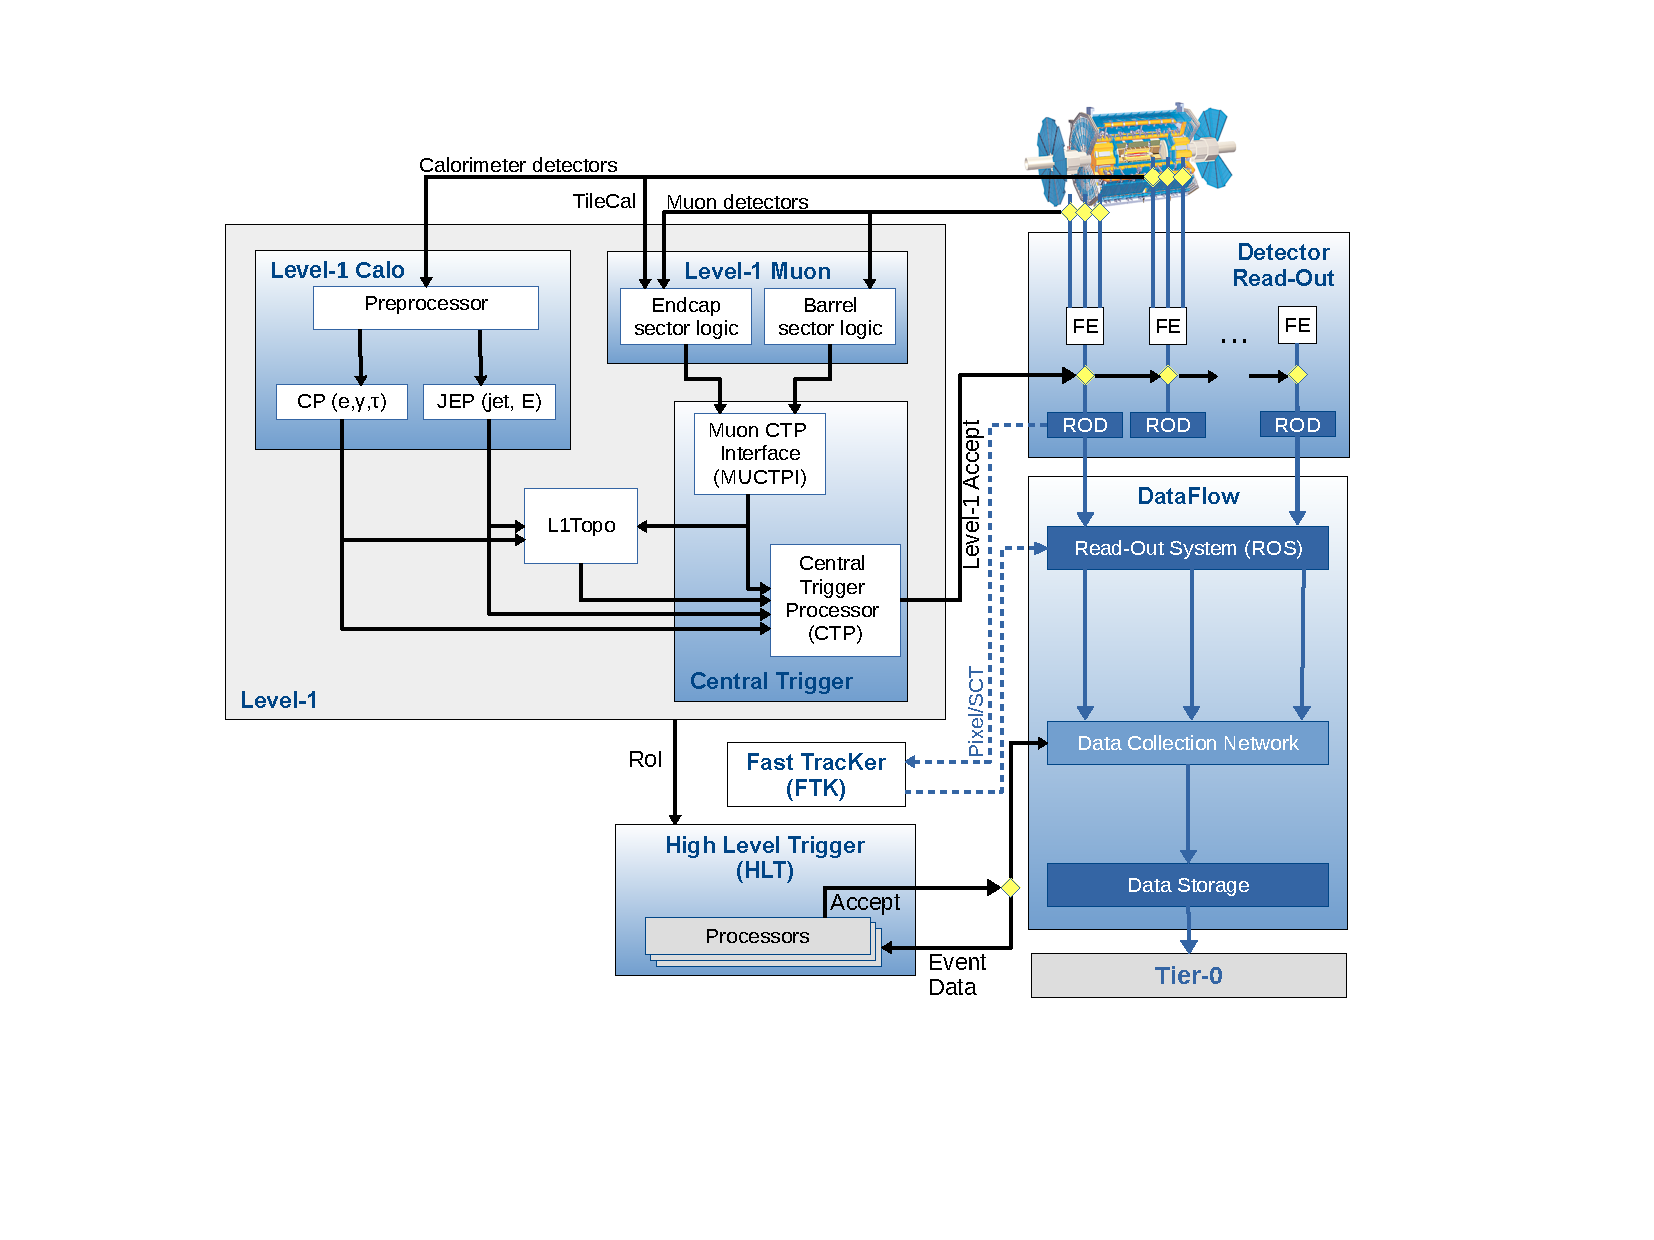
\includegraphics[width=0.90\textwidth]{Figs/CH4/ATLAS_TDAQ.pdf}
    \caption[ATLAS Run-2 trigger and data acquisition system]{
    Schematic overview of the ATLAS Run-2 trigger and data acquisition system~\cite{ATLASTriggerRun2}.
    }
    \label{fig:atlas_tdaq}
\end{figure}

\begin{itemize}
    \item \textbf{\textit{L1 calorimeter trigger~(L1Calo)}}

    L1Calo uses reduced-granularity information from the electromagnetic and hadronic calorimeters to reconstruct energy deposits within the Level-1 latency.
    Signals from neighbouring calorimeter cells are combined into trigger towers in the $(\eta,\phi)$ plane, and dedicated hardware algorithms search for local maxima in the transverse-energy distribution by comparing the energies of neighbouring towers.
    The same calorimeter information is also summed over larger regions to reconstruct jet-like energy deposits and global quantities such as the total and missing transverse energy.

    \item \textbf{\textit{L1 muon trigger~(L1Muon)}}

    L1Muon identifies muon candidates using fast signals from the RPCs and the TGCs. 
    Hits in different trigger-chamber layers are required to form spatial coincidence patterns consistent with a muon trajectory, while their timing information is used to associate the candidate with the correct bunch crossing. 
    The amount of bending in the magnetic field is used to determine whether the candidate satisfies predefined transverse-momentum thresholds.

    \item \textbf{\textit{L1 topological trigger~(L1Topo)}}

    L1Topo receives compact trigger-object information reconstructed by L1Calo and L1Muon, including their transverse momentum or energy and $(\eta,\phi)$ positions.
    Dedicated FPGA hardware combines these objects and calculates event-level topological quantities.
    And these quantities are compared with predefined selection requirements.
\end{itemize}

The trigger decisions from L1Calo, L1Muon, and L1Topo are then sent to the Central Trigger Processor~(CTP), which combines them according to the predefined L1 trigger menu.

If at least one enabled trigger item is satisfied, the CTP issues a Level-1 Accept~(L1A) signal for the corresponding bunch crossing.
The L1A signal is distributed to the detector front-end electronics and initiates the transfer of the detector data associated with that bunch crossing from the front-end buffers to the readout system.

For accepted events, the L1 trigger also provides Regions of Interest~(RoIs), which identify detector regions associated with the trigger objects responsible for the L1 decision.
These RoIs provide seed information for the HLT and allow detailed reconstruction to be performed initially in limited detector regions, reducing the required processing time.

\subsubsection*{High-Level Trigger}

The HLT is the second stage of the ATLAS trigger system.
It is implemented in a large computing farm and runs software algorithms using detector information with substantially finer granularity than is available at L1.
The HLT reconstruction is guided by RoIs identified by the L1 trigger, while full-event reconstruction can also be used for signatures such as jets and missing transverse momentum.
The HLT algorithms are designed to provide reconstruction performance close to that of the offline algorithms while remaining sufficiently fast for online operation.
As a reuslt, the HLT reduced the L1 output rate to an average recording rate of approximately $1~\mathrm{kHz}$ for permanent storage~\cite{ATLASTriggerRun2}.

The trigger menu comprises the active L1 and HLT selections used during data taking with prescale factors, which are applied to selected trigger items to control their rates according to the instantaneous luminosity and available bandwidth.